%%%%%%%%%%%%%%%%%%%%%%%%%%%%%%%%%%%%%%%%%
% Beamer Presentation
% LaTeX Template
% Version 1.0 (10/11/12)
%
% This template has been downloaded from:
% http://www.LaTeXTemplates.com
%
% License:
% CC BY-NC-SA 3.0 (http://creativecommons.org/licenses/by-nc-sa/3.0/)
%
%%%%%%%%%%%%%%%%%%%%%%%%%%%%%%%%%%%%%%%%%

%----------------------------------------------------------------------------------------
%	PACKAGES AND THEMES
%----------------------------------------------------------------------------------------

\documentclass{beamer}

\mode<presentation> {

% The Beamer class comes with a number of default slide themes
% which change the colors and layouts of slides. Below this is a list
% of all the themes, uncomment each in turn to see what they look like.

%\usetheme{default}
% \usetheme{AnnArbor}
%\usetheme{Antibes}
%\usetheme{Bergen}
%\usetheme{Berkeley}
%\usetheme{Berlin}
%\usetheme{Boadilla}
%\usetheme{CambridgeUS}
%\usetheme{Copenhagen}
%\usetheme{Darmstadt}
\usetheme{Dresden}
%\usetheme{Frankfurt}
%\usetheme{Goettingen}
%\usetheme{Hannover}
%\usetheme{Ilmenau}
%\usetheme{JuanLesPins}
%\usetheme{Luebeck}
%\usetheme{Madrid}
%\usetheme{Malmoe}
%\usetheme{Marburg}
%\usetheme{Montpellier}
%\usetheme{PaloAlto}
%\usetheme{Pittsburgh}
%\usetheme{Rochester}
%\usetheme{Singapore}
%\usetheme{Szeged}
%\usetheme{Warsaw}

% As well as themes, the Beamer class has a number of color themes
% for any slide theme. Uncomment each of these in turn to see how it
% changes the colors of your current slide theme.

%\usecolortheme{albatross}
%\usecolortheme{beaver}
%\usecolortheme{beetle}
%\usecolortheme{crane}
%\usecolortheme{dolphin}
%\usecolortheme{dove}
%\usecolortheme{fly}
%\usecolortheme{lily}
%\usecolortheme{orchid}
%\usecolortheme{rose}
%\usecolortheme{seagull}
%\usecolortheme{seahorse}
%\usecolortheme{whale}
%\usecolortheme{wolverine}

%\setbeamertemplate{footline} % To remove the footer line in all slides uncomment this line
%\setbeamertemplate{footline}[page number] % To replace the footer line in all slides with a simple slide count uncomment this line

%\setbeamertemplate{navigation symbols}{} % To remove the navigation symbols from the bottom of all slides uncomment this line
}

\usepackage{graphicx} % Allows including images
\usepackage{booktabs} % Allows the use of \toprule, \midrule andxs                      % \bottomrule in tables
\usepackage{float}
\usepackage{caption}
\usepackage{subcaption}
\usepackage{listings} %syntax highlighting?
\usepackage{minted}
%\usepackage{subfigure}

%----------------------------------------------------------------------------------------
%	TITLE PAGE
%----------------------------------------------------------------------------------------

\title[How do I SimpleCV?]{A Crash Course on SimpleCV} % The short title appears at the bottom of every slide, the full title is only on the title page

\author{Katherine Scott} % Your name
%\author{Anthony Oliver} % Your name

\institute[SightMachine] % Your institution as it will appear on the bottom of every slide, may be shorthand to save space
{
SightMachine \\ % Your institution for the title page
\medskip
\textit{kat@sightmachine.com}
\textit{anthony@sightmachine.com} % Your email address
}
\date{\today} % Date, can be changed to a custom date

\begin{document}

\begin{frame}
\titlepage % Print the title page as the first slide
\end{frame}

\begin{frame}
\frametitle{Overview} % Table of contents slide, comment this block out to remove it
\tableofcontents % Throughout your presentation, if you choose to use \section{} and \subsection{} commands, these will automatically be printed on this slide as an overview of your presentation
\end{frame}

%----------------------------------------------------------------------------------------
%	PRESENTATION SLIDES
%----------------------------------------------------------------------------------------
\section{Quick Start!}
 \begin{frame}
   \frametitle{Get Started!}
   There are a lot of dependencies for SimpleCV and it is a bit tough for
   beginners. We've brought disks that are ready to go!
   \begin{itemize}
     \item Windows / Linux
       \begin{itemize}
         \item Boot from USB drive.
         \item Alternatively install VirtualBox and the image. 
         \item \url{https://www.virtualbox.org/}
         \end{itemize}
     \item Macs 
       \begin{itemize}
         \item Newer macs are persnikety about booting from a USB drive.
         \item Install virtual box and the ISO and go to town. 
         \end{itemize}
     \item When you get home install from SuperPack or preferably source libs.
       \begin{itemize}
         \item take awhile and is not a perfect science.
         \item \url{https://github.com/ingenuitas/SimpleCV}
         \item If you want to contribute this is a great place to start.
         \end{itemize}
    \end{itemize}
 \end{frame}

%----------------------------------------------------------------------------------------
\begin{frame}
  \frametitle{About the tutorial}
  \begin{itemize}
    \item It will be a lot of live coding. I'll lead, you follow along.
    \item If you have a question feel free to interrupt. 
    \item If you are having an issue raise a flag. Anthony will help
      you. 
    \end{itemize}
\end{frame}


%------------------------------------------------
\section{What is SimpleCV?} % Sections can be created in order to organize your presentation into discrete blocks, all sections and subsections are automatically printed in the table of contents as an overview of the talk
%------------------------------------------------

\subsection{What makes up SimpleCV?} % A subsection can be created just before a set of slides with a common theme to further break down your presentation into chunks

% ------------------------------------------------
\begin{frame}
\frametitle{What Makes Up SimpleCV?}
\begin{figure}

\includegraphics[width=0.5\linewidth]{simplecv.png}
\end{figure}
\end{frame}

% ------------------------------------------------

\begin{frame}
\frametitle{SimpleCV != OpenCV }
\begin{figure}
  
\includegraphics[width=0.2\linewidth]{simplecv.png}
\end{figure}
\begin{itemize}
  \item OpenCV is really busy, we help by wrapping python.
  \item We add lots of other fun stuff (OCR, Barcodes, etc.)
  \item We are not competing, we are complementing. 
  \item Purposes are different. Python is great for prototyping. C++ great for embedded.
\end{itemize}
\end{frame}

% ------------------------------------------------

\begin{frame}
  \frametitle{Core Dependencies}
  \begin{itemize}
  \item \href{http://www.opencv.org}{OpenCV} Python Bindings
  \item \href{http://docs.scipy.org/doc/}{Numpy}
  \item \href{http://docs.scipy.org/doc/}{SciPy}
  \item SciKits Learn and \href{http://orange.biolab.si/}{Orange}
  \item \href{http://www.pygame.org}{PyGame} (this is going away)
  \item \href{http://www.pythonware.com/products/pil/}{Python Imaging Library (PIL)}
  \item \href{http://ipython.org/}{ipython}
  \item PIL (Python Imaging Library)
  \end{itemize}
\end{frame}

% ------------------------------------------------

\begin{frame}
  \frametitle{Optional Dependencies}
  \begin{itemize}
  \item Barcodes- Zebra Crossing \href{https://code.google.com/p/zxing/}{ZXIng}
  \item Optical Character Recognition (OCR) - \href{https://code.google.com/p/tesseract-ocr/}{Tesseract}
  \item Beautiful Soup 
  \item Kinect Support - freenect 
  \item Unit Tests - nose
  \item Web Stuff - flask / CherryPy
  \item Arduino - pyfirmata
  \item Many Many Many more. 
  \end{itemize}
\end{frame}

% ------------------------------------------------

\begin{frame}
  \frametitle{This is why we put everything in a superpack / virtual
    box / bootable drive}
  \begin{itemize}
  \item Just get to the core library functions.
  \item We encourage you to install the full library when you get
    home.
  \item Help is available if you need it. 
  \end{itemize}
\end{frame}

% ------------------------------------------------
\begin{frame}
\frametitle{Getting Help after the tutorial.}
\begin{figure}
  
\includegraphics[width=0.2\linewidth]{hang-in-there-cat.jpg}
\end{figure}
\begin{itemize}
  \item Primary Source: \url{http://help.simplecv.org/questions/}
  \item Documentation \url{http://www.simplecv.org/docs/}
  \item Tweet at us: $@$Simple\textunderscore CV
  \item Another Good Resource: \url{http://www.reddit.com/r/ComputerVision}
\end{itemize}
\end{frame}

% ------------------------------------------------
\begin{frame}
\frametitle{On the Printed Page}

 \begin{figure}
%   \begin{subfigure}
     
\includegraphics[width=0.4\linewidth]{SimpleCVBook.jpg}
%   \end{subfigure}
%   \begin{sub-figure}
     \quad
     
\includegraphics[width=0.4\linewidth]{JanEricBook.jpg}
     \caption{Two books about using Python for Computer Vision}
%   \end{subfigure}
 \end{figure}

\end{frame}

% ------------------------------------------------
\begin{frame}
\frametitle{So why are we doing this?}

\begin{itemize}
  \item We are really nice people who believe in Python and Open
    Source.
  \item We are trying to disrupt industrial quality control systems.
\end{itemize}
\begin{figure}
  
\includegraphics[width=0.6\linewidth]{SightMachineLogo.png}
\end{figure}

\end{frame}

% ------------------------------------------------
\begin{frame}
\frametitle{Early Prototypes}

\begin{figure}
  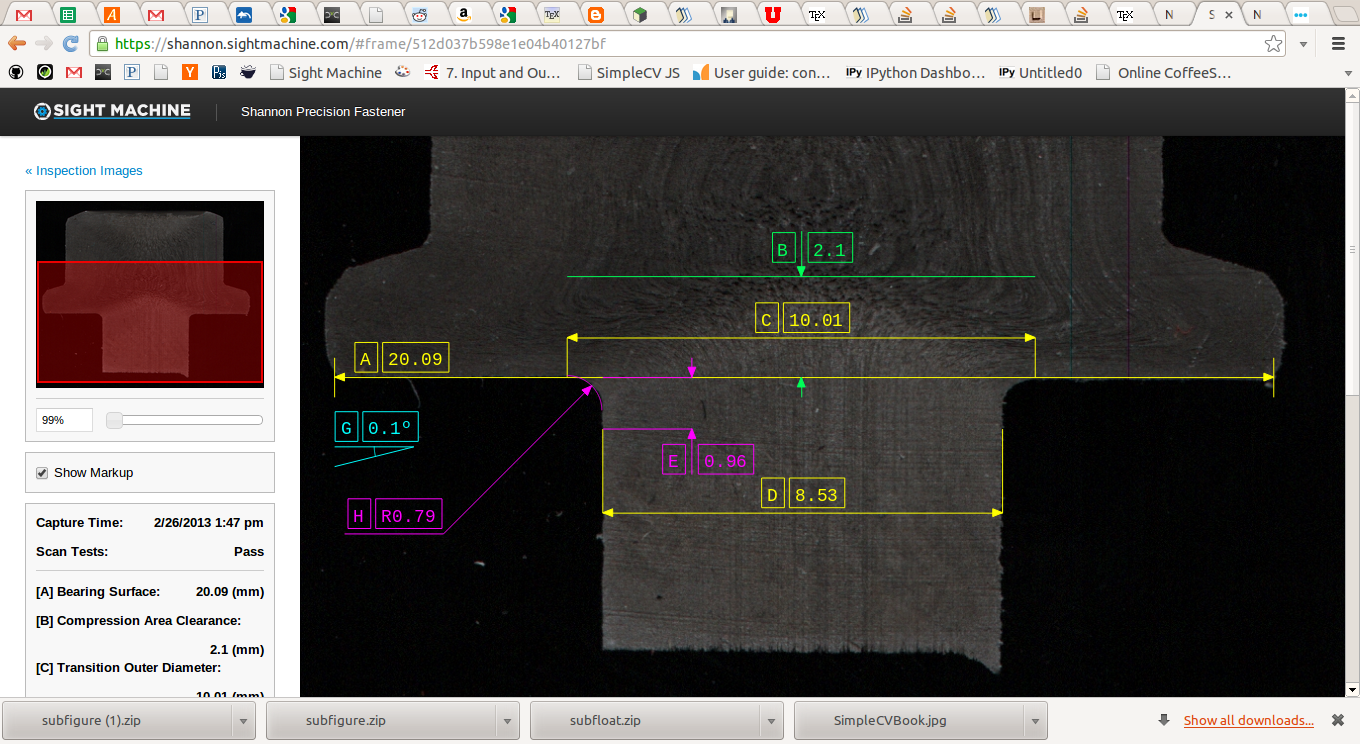
\includegraphics[width=0.9\linewidth]{shannon.png}
  \caption{Early Customer - Industrial Fastener Morphology
      and Metallurgy }
\end{figure}

\end{frame}
% ------------------------------------------------
\begin{frame}
\frametitle{Early Prototypes}

\begin{figure}
  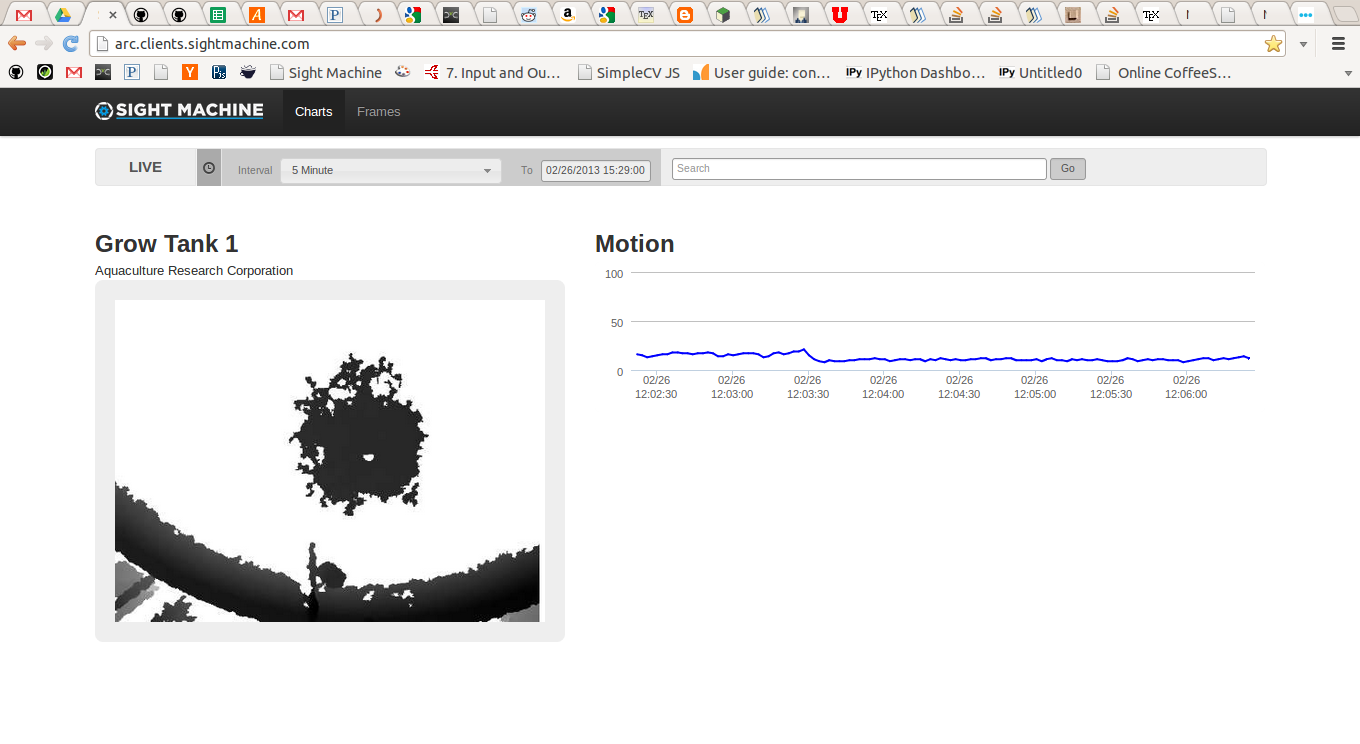
\includegraphics[width=0.9\linewidth]{arc.png}
  \caption{Early Customer - Aquaponics Research Facility}
\end{figure}

\end{frame}

\section{SimpleCV}
\subsection{Getting Started}

% ------------------------------------------------
\begin{frame}
\frametitle{How do I SimpleCV?}

\begin{figure}
  
\includegraphics[width=0.7\linewidth]{howdoi.jpg}
\end{figure}

\end{frame}

 
% ------------------------------------------------
\begin{frame}
  \frametitle{Paragraphs of Text}
  Sed iaculis dapibus gravida. Morbi sed tortor erat, nec interdum arcu. Sed id lorem lectus. Quisque viverra augue id sem ornare non aliquam nibh tristique. Aenean in ligula nisl. Nulla sed tellus ipsum. Donec vestibulum ligula non lorem vulputate fermentum accumsan neque mollis.\\~\\

  Sed diam enim, sagittis nec condimentum sit amet, ullamcorper sit
  amet libero. Aliquam vel dui orci, a porta odio. Nullam id suscipit
  ipsum. Aenean lobortis commodo sem, ut commodo leo gravida
  vitae. Pellentesque vehicula ante iaculis arcu pretium rutrum eget
  sit amet purus. Integer ornare nulla quis neque ultrices
  lobortis. Vestibulum ultrices tincidunt libero, quis commodo erat
  ullamcorper id.
\end{frame}

% ------------------------------------------------

\begin{frame}
  \frametitle{Bullet Points}
  \begin{itemize}
  \item Lorem ipsum dolor sit amet, consectetur adipiscing elit
  \item Aliquam blandit faucibus nisi, sit amet dapibus enim tempus eu
  \item Nulla commodo, erat quis gravida posuere, elit lacus lobortis
    est, quis porttitor odio mauris at libero
  \item Nam cursus est eget velit posuere pellentesque
  \item Vestibulum faucibus velit a augue condimentum quis convallis
    nulla gravida
  \end{itemize}
\end{frame}

% ------------------------------------------------

\begin{frame}
  \frametitle{Multiple Columns}

  \begin{columns}[c] % The "c" option specifies centered vertical alignment while the "t" option is used for top vertical alignment

    \column{.45\textwidth} % Left column and width
    \textbf{Heading}
    \begin{enumerate}
    \item Statement
    \item Explanation
    \item Example
    \end{enumerate}

    \column{.5\textwidth} % Right column and width
    Lorem ipsum dolor sit amet, consectetur adipiscing elit. Integer
    lectus nisl, ultricies in feugiat rutrum, porttitor sit amet
    augue. Aliquam ut tortor mauris. Sed volutpat ante purus, quis
    accumsan dolor.

  \end{columns}
\end{frame}

% ------------------------------------------------
\section{Second Section}
%------------------------------------------------

\begin{frame}
\frametitle{Table}
\begin{table}
\begin{tabular}{l l l}
\toprule
\textbf{Treatments} & \textbf{Response 1} & \textbf{Response 2}\\
\midrule
Treatment 1 & 0.0003262 & 0.562 \\
Treatment 2 & 0.0015681 & 0.910 \\
Treatment 3 & 0.0009271 & 0.296 \\
\bottomrule
\end{tabular}
\caption{Table caption}
\end{table}
\end{frame}

%------------------------------------------------

\begin{frame}
\frametitle{Theorem}
\begin{theorem}[Mass--energy equivalence]
$E = mc^2$
\end{theorem}
\end{frame}

%------------------------------------------------


\begin{frame}[fragile] % Need to use the fragile option when verbatim is used in the slide
\frametitle{Verbatim}
\begin{example}[Theorem Slide Code]
\begin{minted}{python}

  def doStuff(a,b,c=[1,2,3]):
      a = 5
      b = a 
      c.reverse()
  
  derp = [1,2,3,4]
  for i in derp:
     doStuff()
     pass
  print derp

\end{minted}
\end{example}
\end{frame}


\begin{frame}[fragile] % Need to use the fragile option when verbatim is used in the slide
\frametitle{Verbatim}
\begin{example}[Theorem Slide Code]
\begin{verbatim}

$E = mc^2$

\end{verbatim}
\end{example}
\end{frame}

%------------------------------------------------

\begin{frame}
\frametitle{Figure}
Uncomment the code on this slide to include your own image from the same directory as the template .TeX file.
%\begin{figure}
%\includegraphics[width=0.8\linewidth]{test}
%\end{figure}
\end{frame}

%------------------------------------------------

\begin{frame}[fragile] % Need to use the fragile option when verbatim is used in the slide
\frametitle{Citation}
An example of the \verb|\cite| command to cite within the presentation:\\~

This statement requires citation \cite{p1}.
\end{frame}

%------------------------------------------------

\begin{frame}
\frametitle{References}
\footnotesize{
\begin{thebibliography}{99} % Beamer does not support BibTeX so references must be inserted manually as below
\bibitem[Smith, 2012]{p1} John Smith (2012)
\newblock Title of the publication
\newblock \emph{Journal Name} 12(3), 45 -- 678.
\end{thebibliography}
}
\end{frame}

%------------------------------------------------

\begin{frame}
\Huge{\centerline{The End}}
\end{frame}

%----------------------------------------------------------------------------------------

\end{document} 
